\section{Analyse et conception}
On fait suivre sur les pages suivantes les différents diagrammes.
\subsection{Diagramme de cas d'utilisation}


Avant tout projet, un diagramme de cas d'utilisation permet de bien se rendre compte des besoins utilisateurs pour ne pas oublier certaines fontionnalités. Ce diagramme est général, il convient donc aux trois exercices du sujet.

\subsection{Diagramme de classe}

Pour pouvoir implémenter nos classes en Java, il est plus que nécessaire de concevoir un diagramme de classe.

\subsection{Diagramme d'activité}
Un diagramme d'activité est aussi intéressant pour comprendre le focntionnement de l'application.

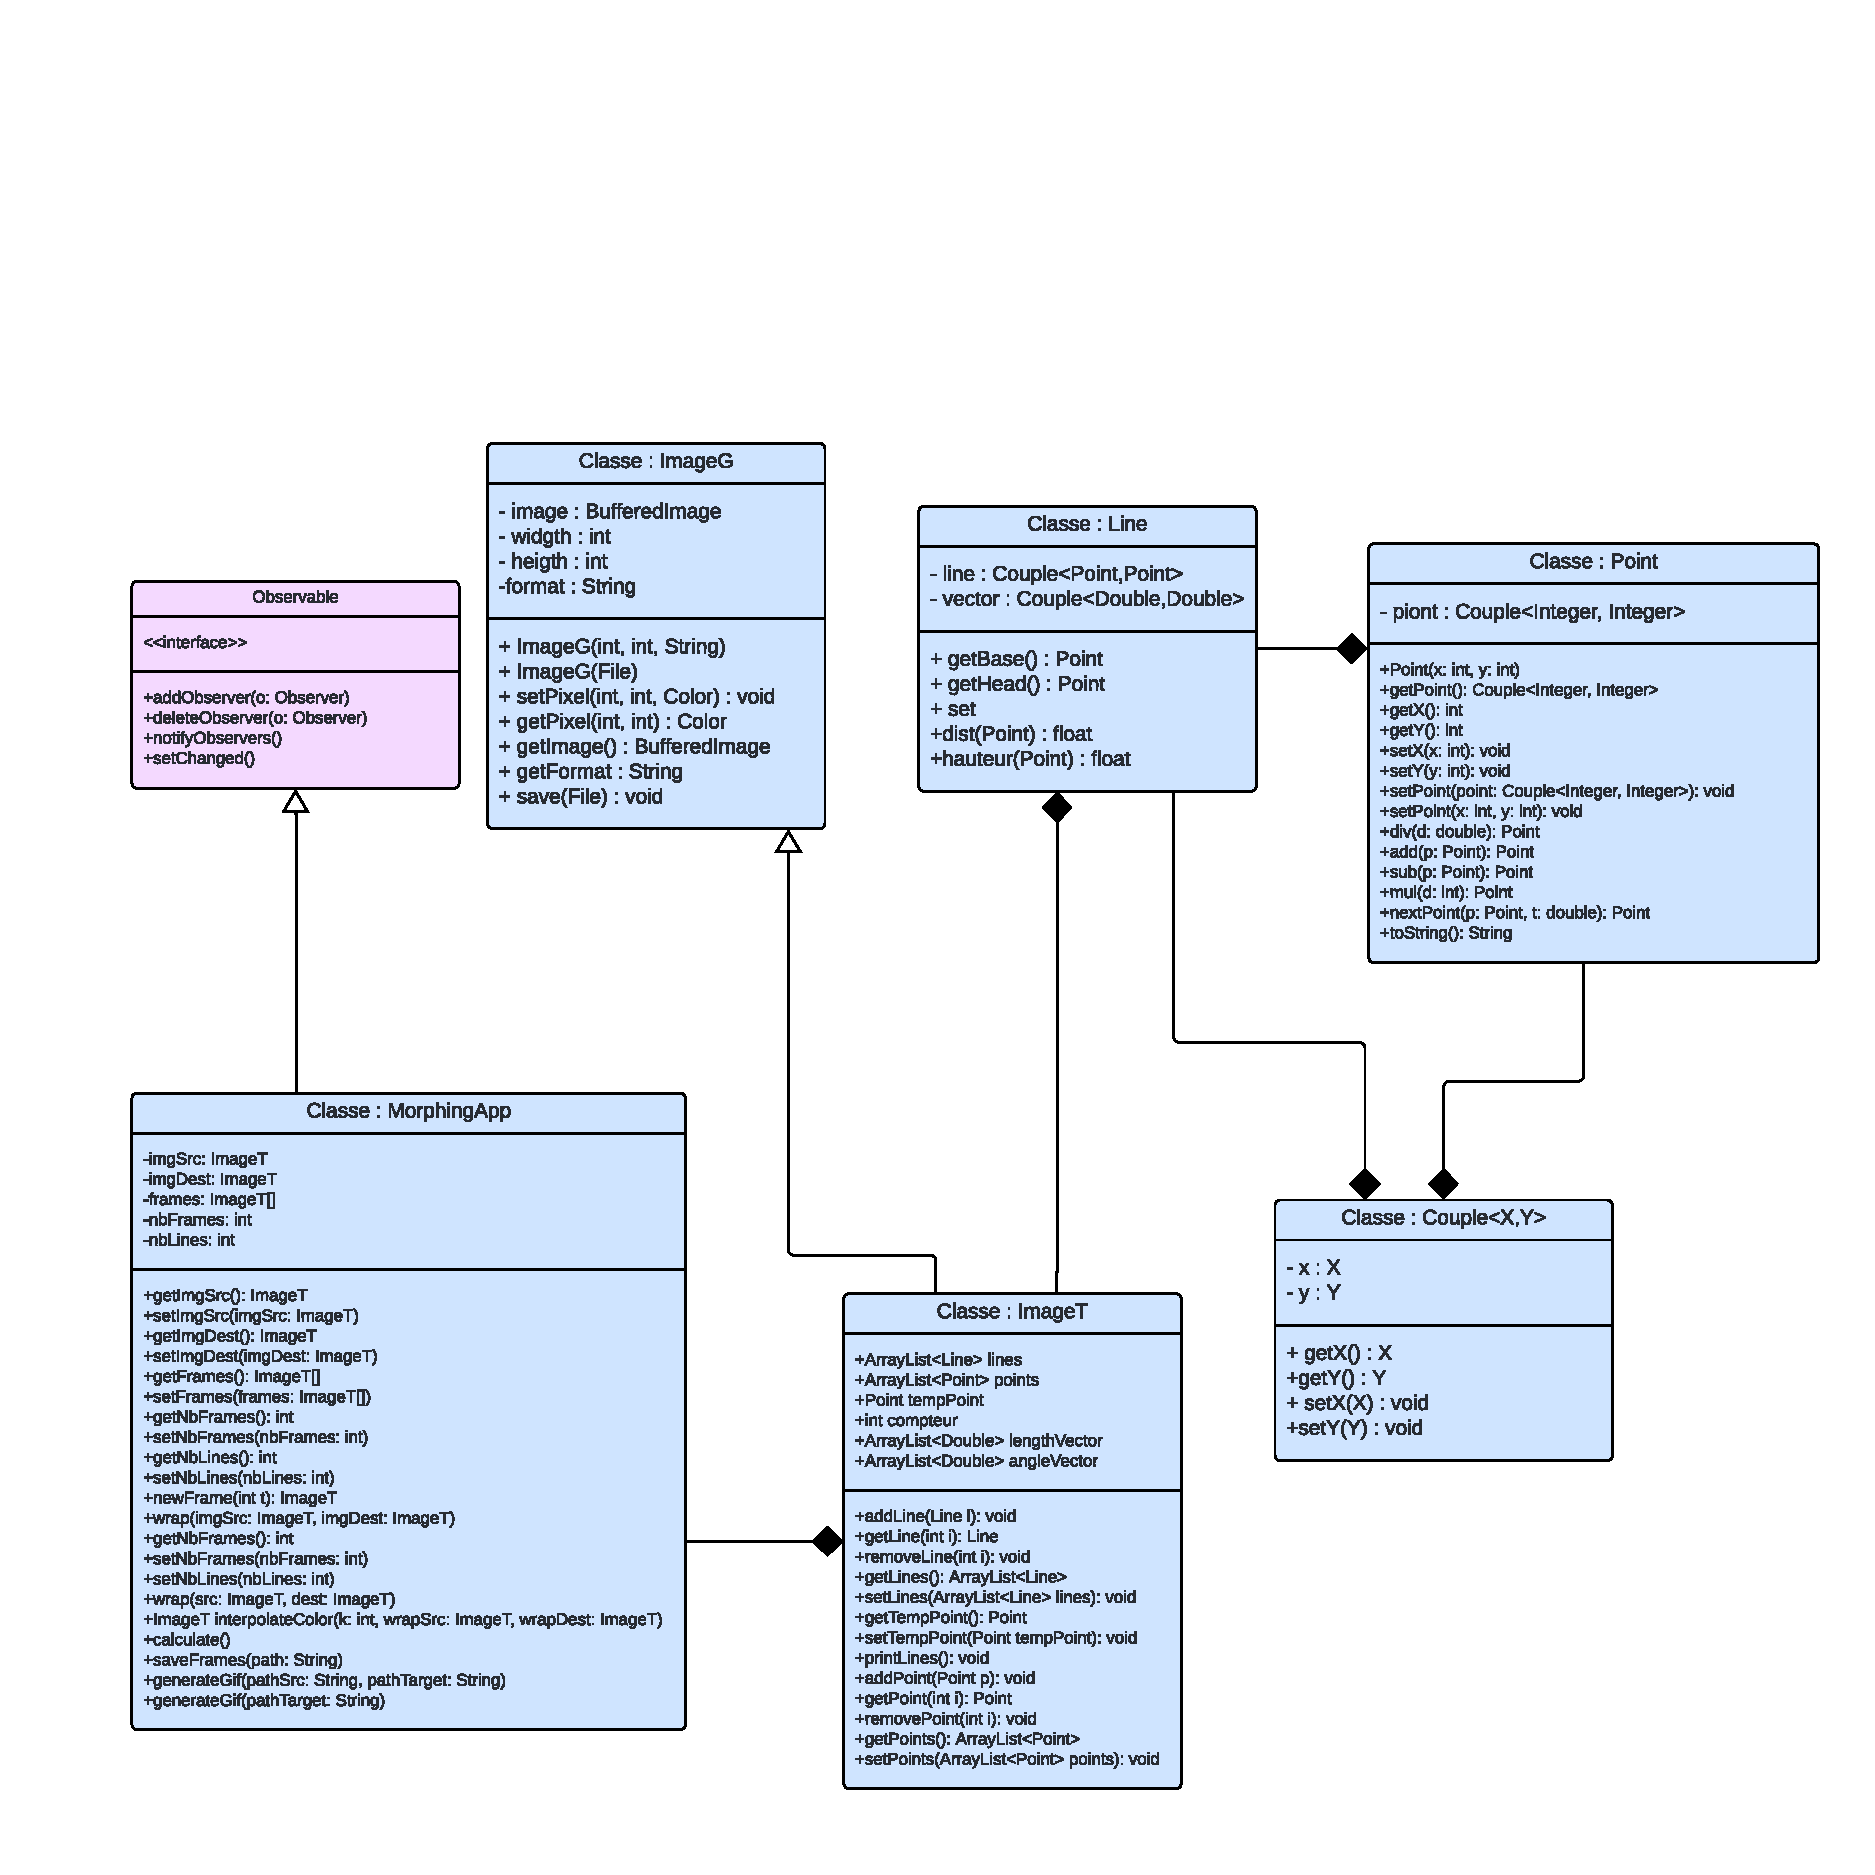
\includepdf[pages={1},fitpaper=true, pagecommand={},]{/home/cytech/Desktop/Morphing/Morphing/rapport/img/diag/MorphingApp-1.pdf}
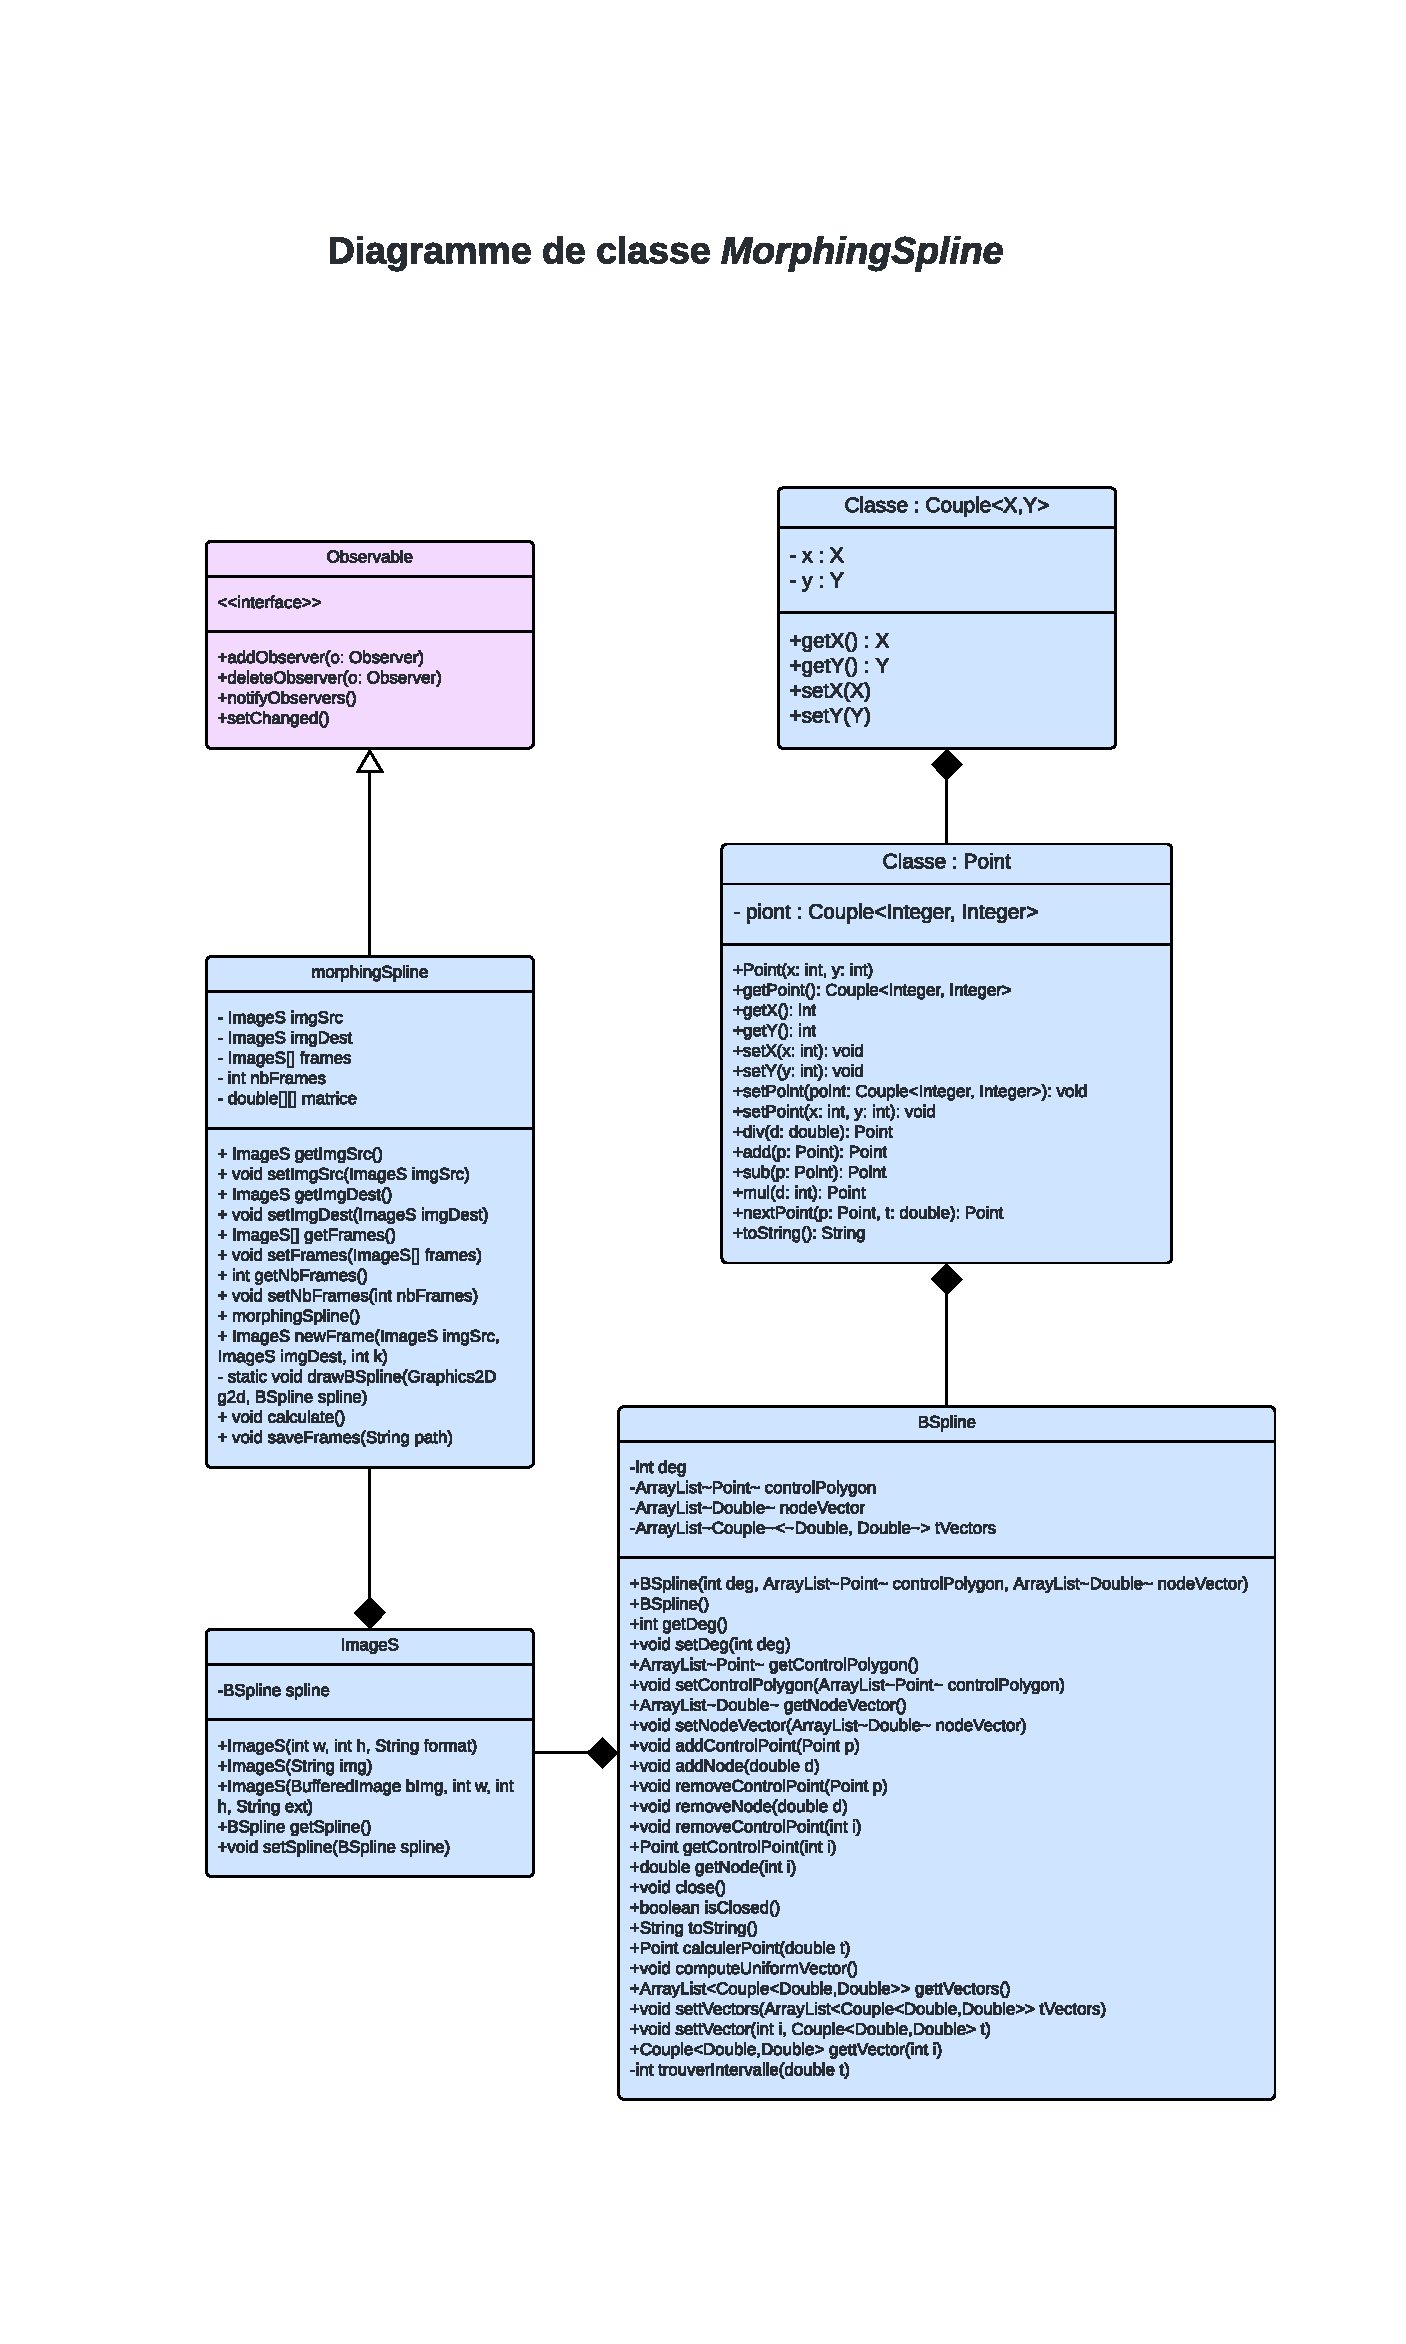
\includepdf[pages={1},fitpaper=true, pagecommand={}]{/home/cytech/Desktop/Morphing/Morphing/rapport/img/diag/Diagramme_vierge-1-1.pdf}
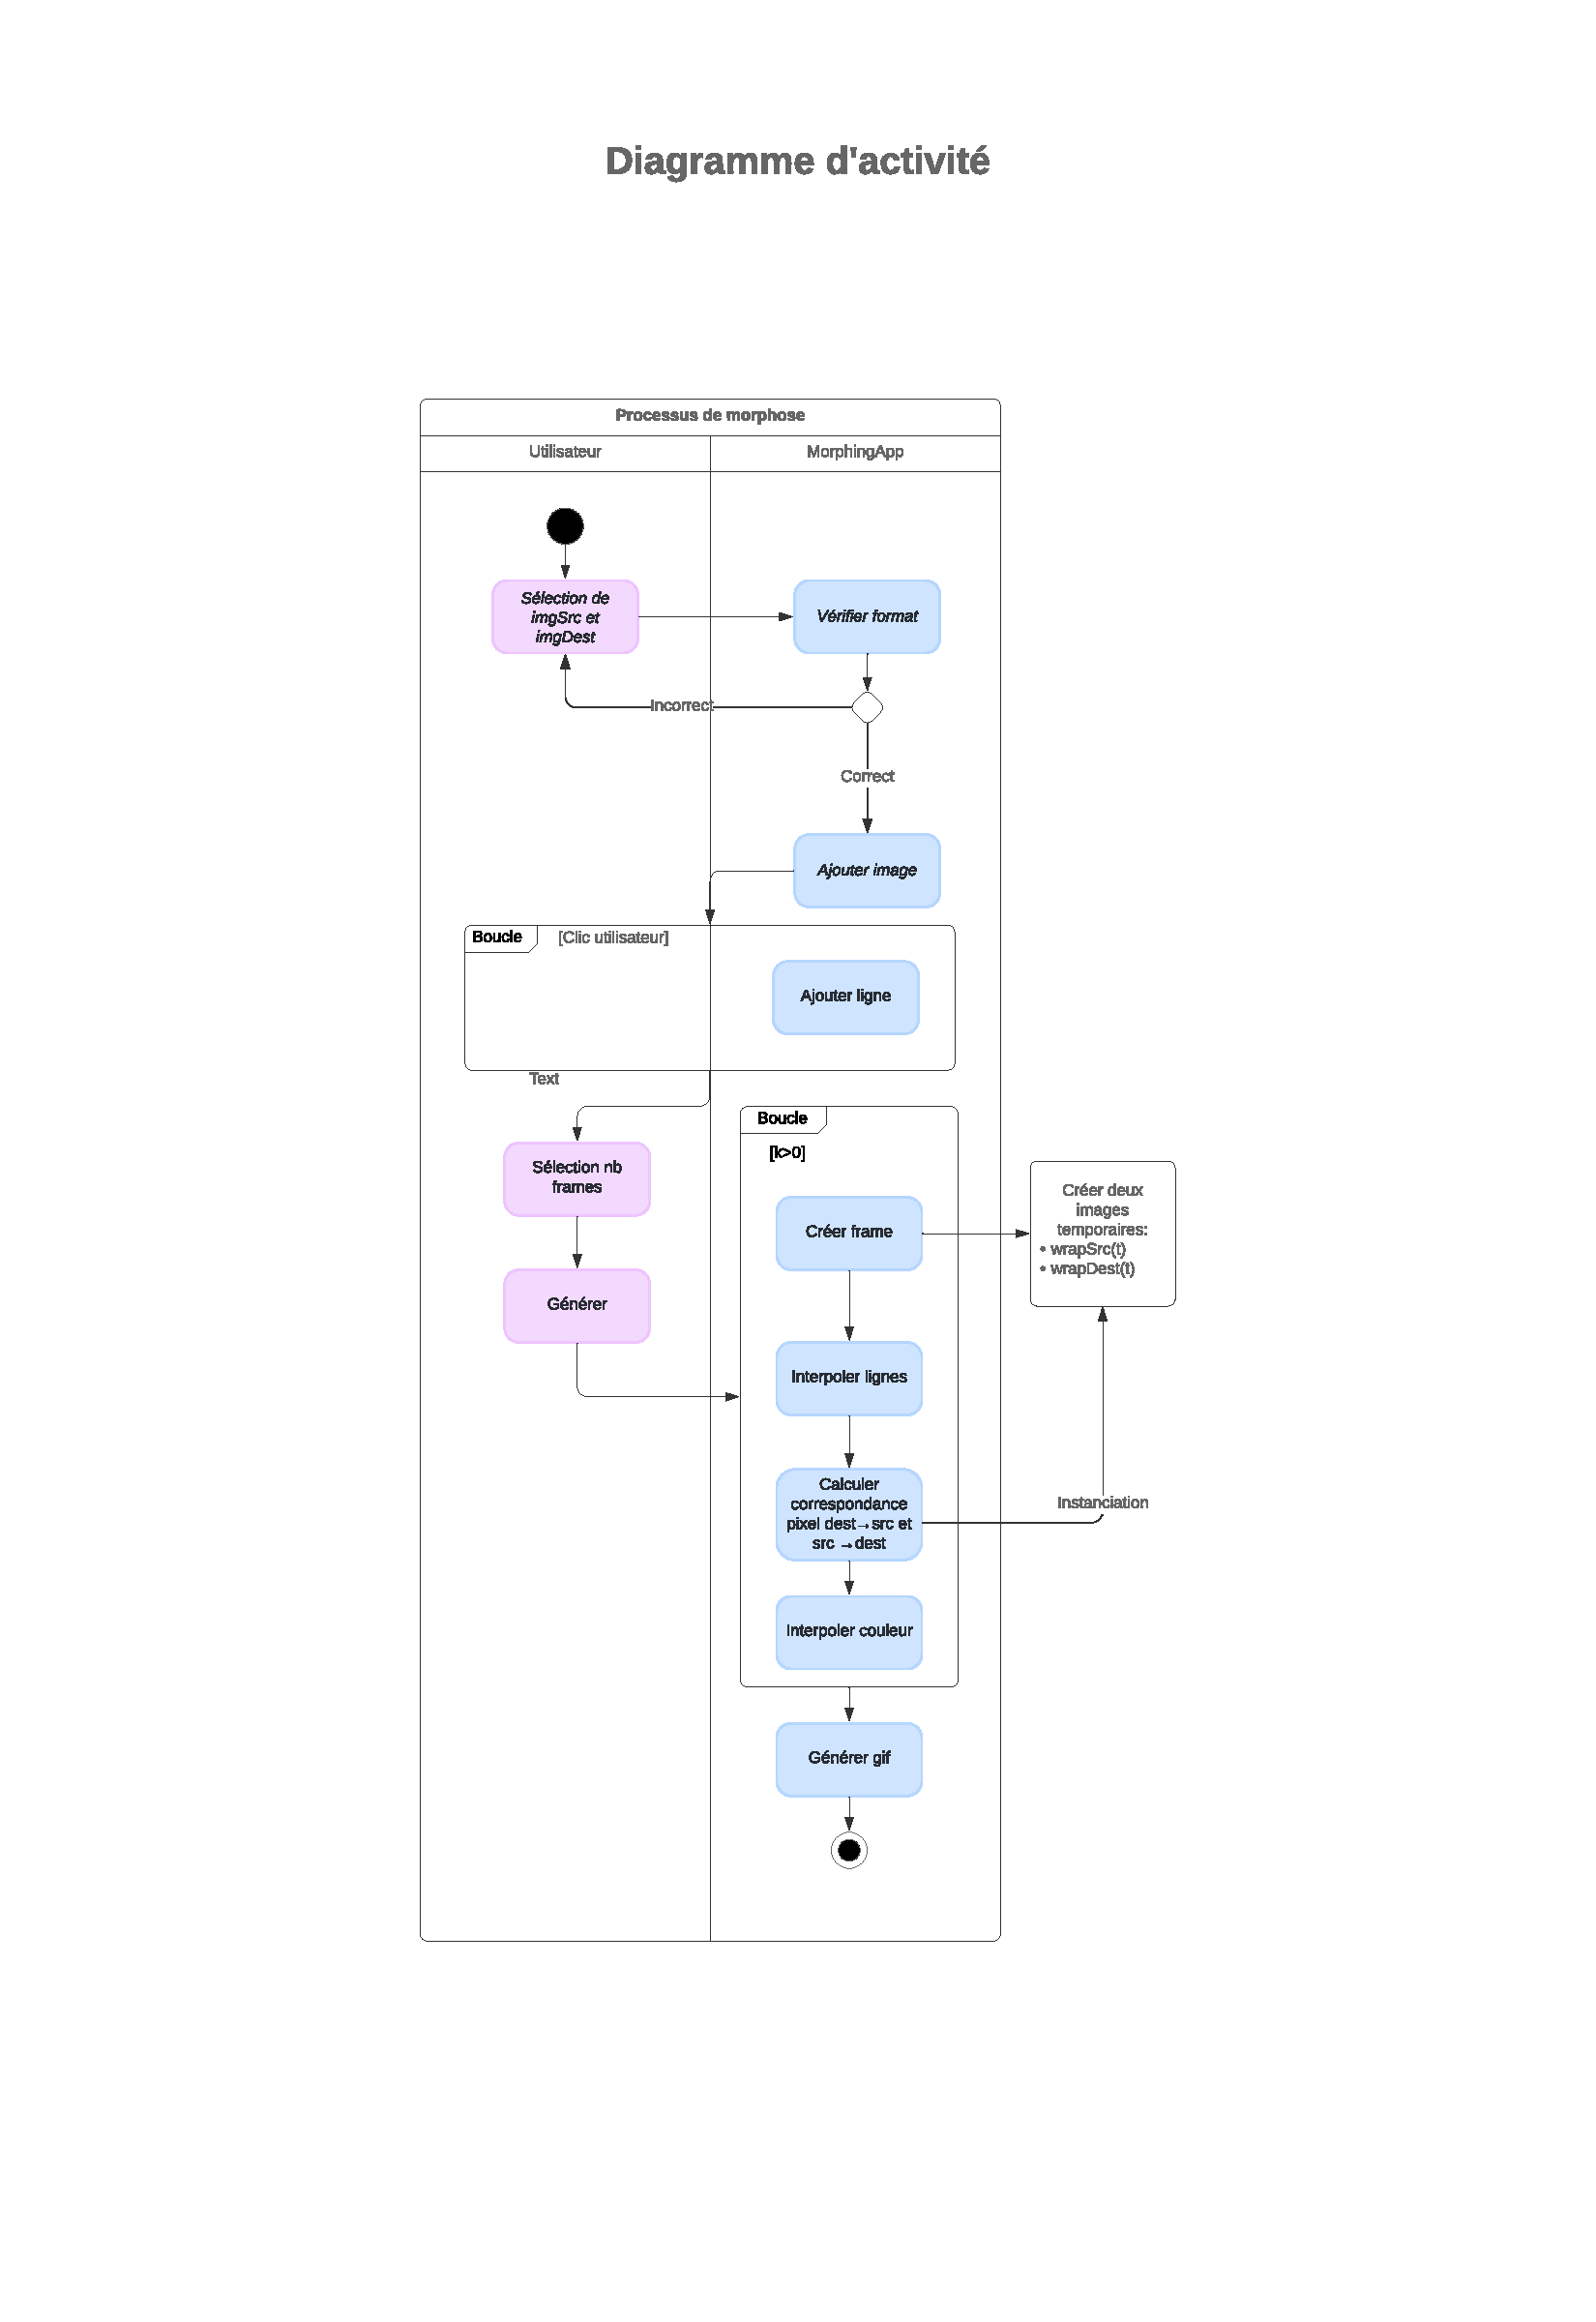
\includepdf[pages={1},fitpaper=true, pagecommand={}]{/home/cytech/Desktop/Morphing/Morphing/rapport/img/diag/Diagramme_dactivites.pdf}
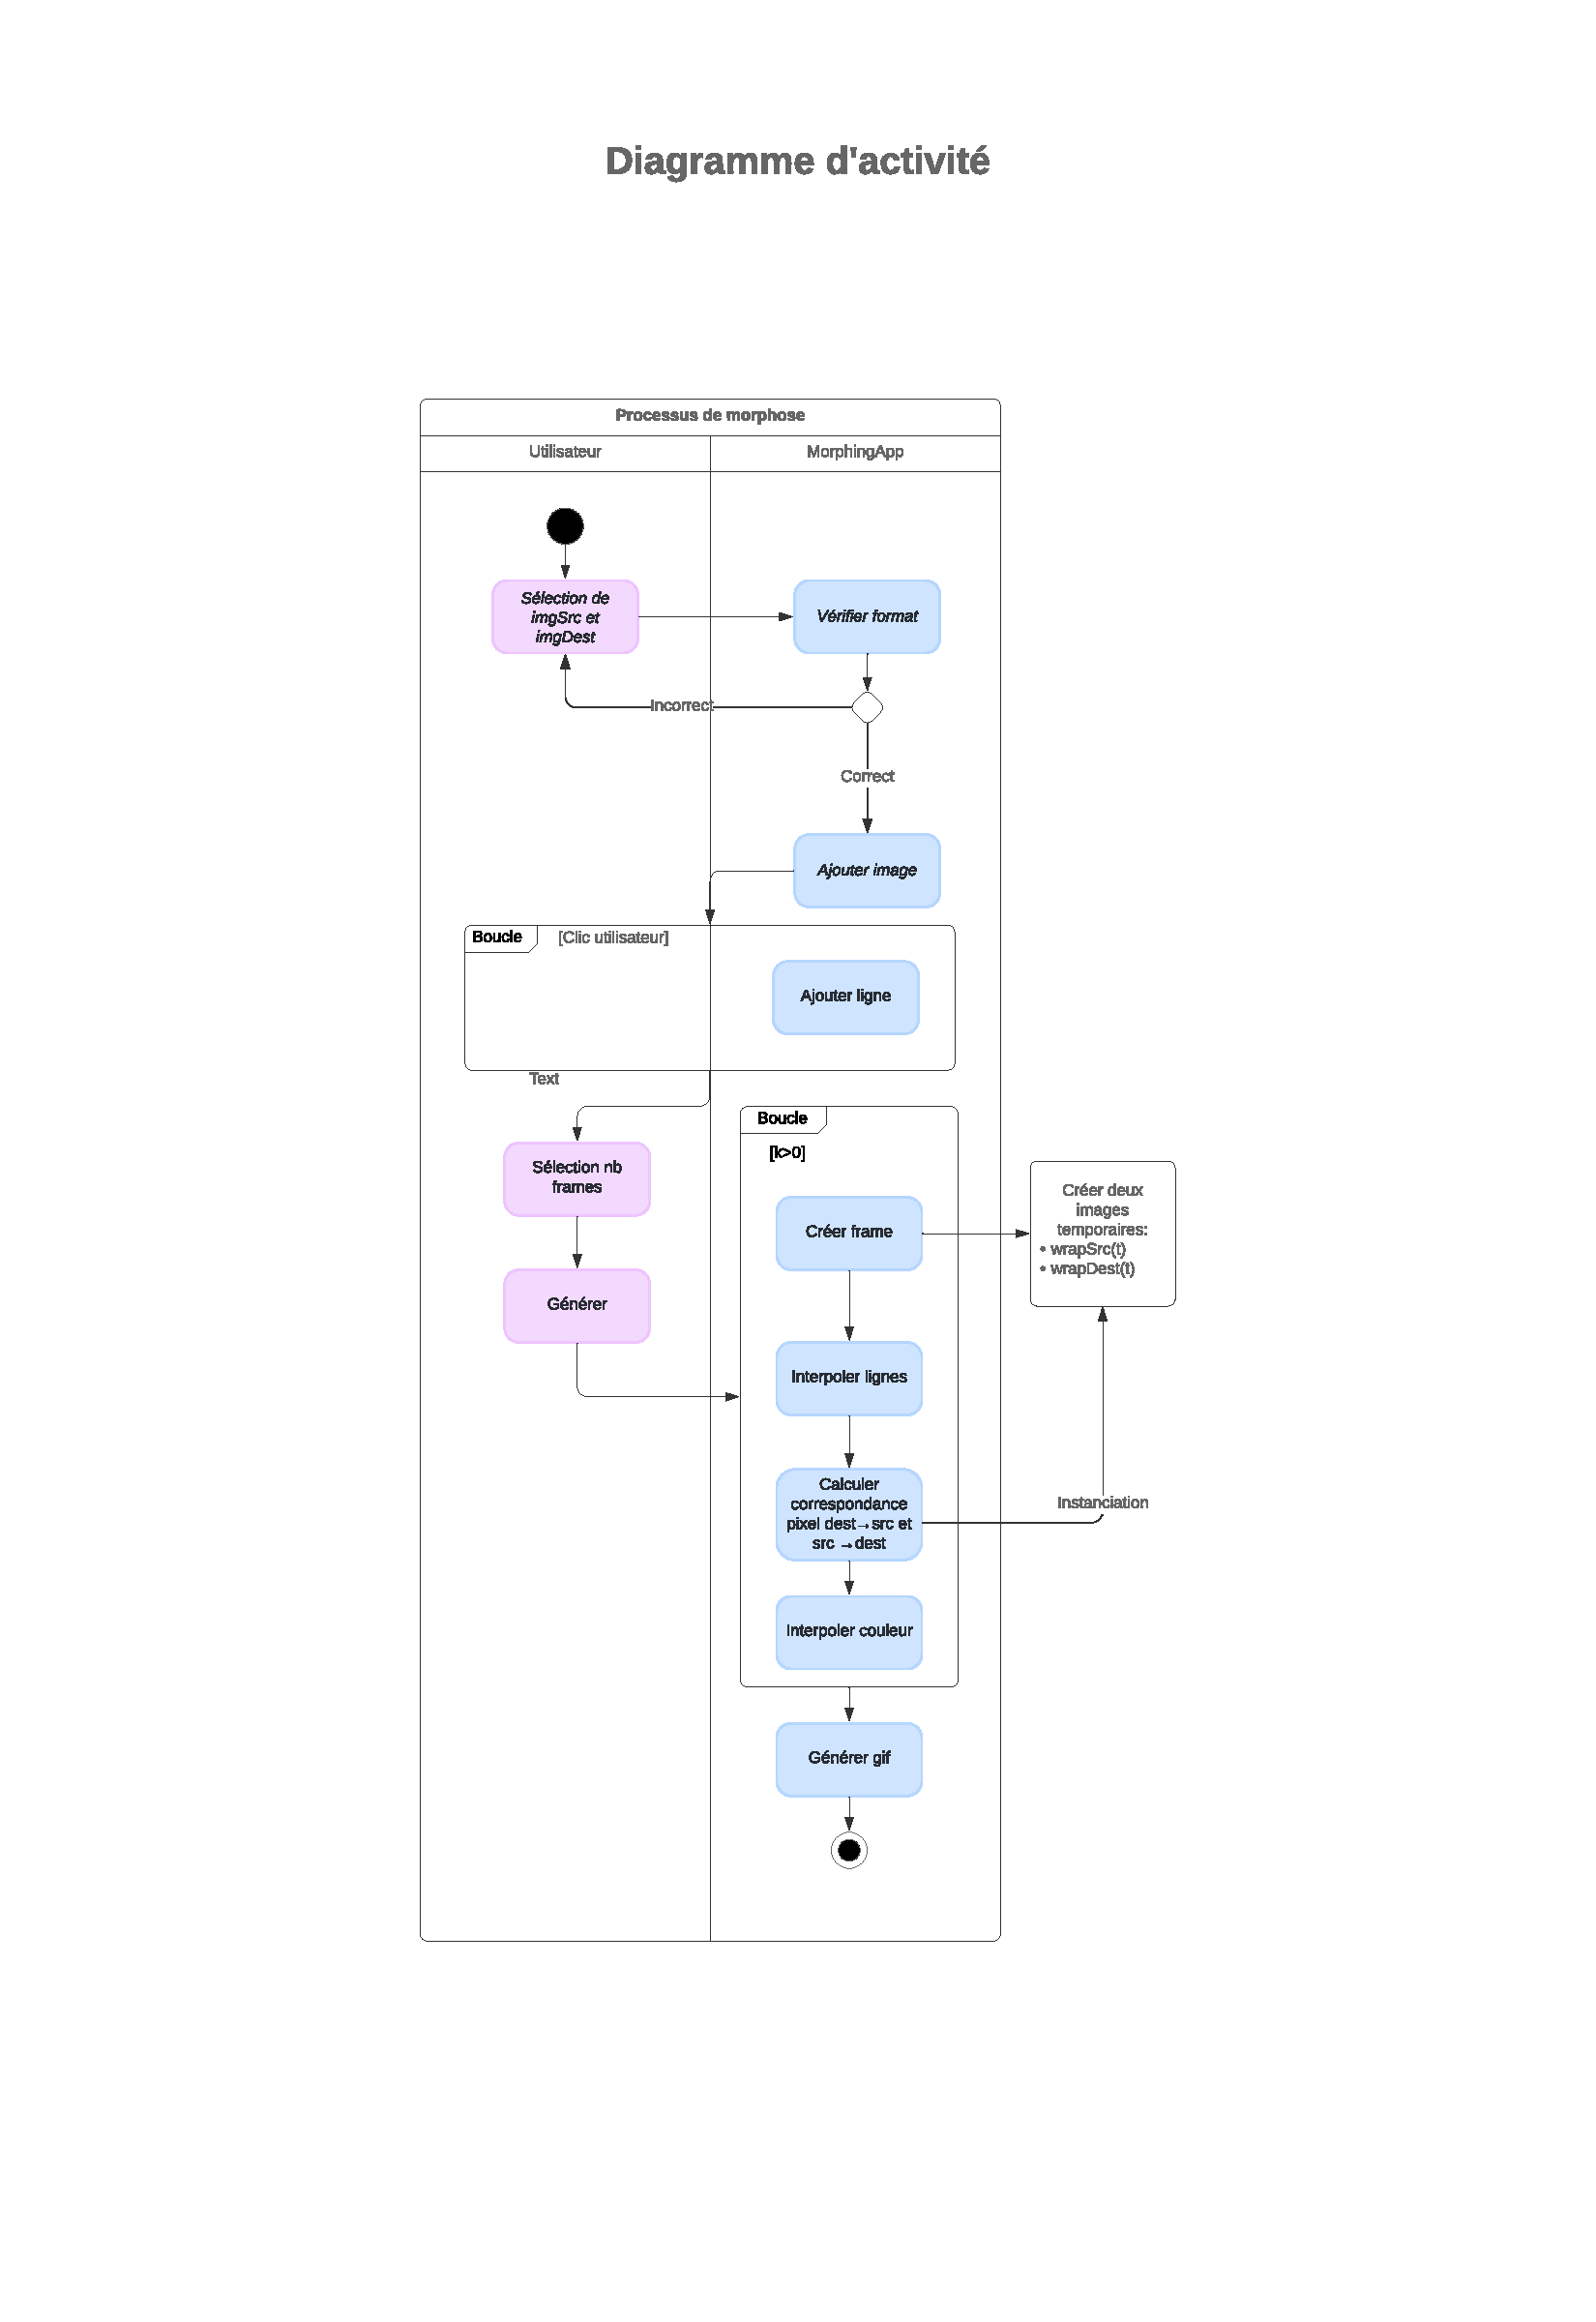
\includepdf[pages={1},fitpaper=true, pagecommand={}]{/home/cytech/Desktop/Morphing/Morphing/rapport/img/diag/Diagramme_dactivites.pdf}






